\section{High Energy}
\subsection{Questions}
\begin{enumerate}
\item \textbf{Describe the mechanisms by which cosmic rays gain and lose energy. Which mechanisms
      are appropriate to which type of particle? Which ones produce electromagnetic
      radiation that we can observe, and in what wave bands?}

      \begin{figure}[ht]
      \centering
      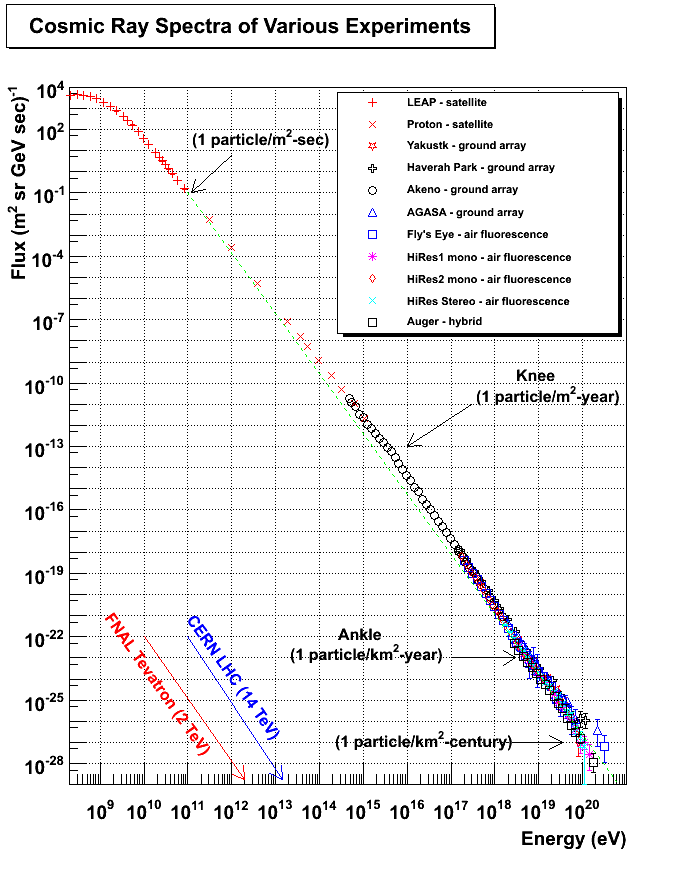
\includegraphics[width=\textwidth]{highenergy_cosmic_ray_spectrum}
      \caption{The ``specific intensity'' of cosmic rays as a function of energy.  Although this
               is almost a perfect power law over 11 orders of magnitude (!), there are two
               important features: the knee at $10^{15}~{\rm eV}$ and the ankle at $10^{18}~{\rm eV}$.}
      \label{fig:cosmic_ray_spectrum}
      \end{figure}

      \newthought{Let's begin by} discussing a few properties of cosmic rays.  At the top of
      the atmosphere, 98\% of cosmic rays are protons and nuclei, while 2\% are electrons.
      Of the protons and nuclei, 87\% are protons, 12\% are helium nuclei, and the remaining
      1\% are more massive nuclei.
      See Figure~\ref{fig:cosmic_ray_spectrum} for the differential energy spectrum at the top of the
      atmosphere (interactions with the atmosphere can produce secondary cosmic rays).
      For protons and nuclei we have
      \begin{dmath}
        N(E)\,\d E \approx 1.8\times10^4\,\left(\frac{E}{\rm GeV}\right)^{-2.7}
                           \,\d E\,{\rm nucleons}\,{\rm m}^{-2}\,{\rm s}^{-1}\,{\rm sr}^{-1}
      \end{dmath},
      while for electrons we have
      \begin{dmath}
        N(E)\,\d E \approx 700\,\left(\frac{E}{\rm GeV}\right)^{-3.3}
                           \,\d E\,{\rm nucleons}\,{\rm m}^{-2}\,{\rm s}^{-1}\,{\rm sr}^{-1}
      \end{dmath}.
      The steeper power law for electrons reflects the fact that electrons are less massive
      and hence lose energy more easily.

      \begin{figure}[ht]
      \centering
      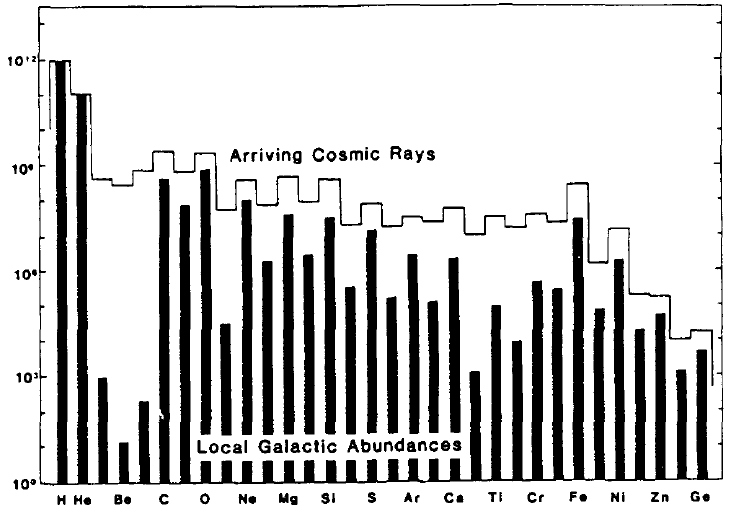
\includegraphics[width=\textwidth]{highenergy_cosmic_ray_abundances}
      \caption{The elemental abundances seen in cosmic rays compared with the local galaxy.
               Note the overabundances of lithium, beryllium, and boron.  A similar
               overabundance is seen near titanium.  The pattern of even elements being more
               common than odd elements (due to the alpha capture process in stars) is seen to
               a lesser extent.  The abundance of heavy elements is remarkably flat.}
      \label{fig:cosmic_ray_abundances}
      \end{figure}

\item \textbf{Discuss the equation of state of relativistic/nonrelativistic degenerate gases of electrons
      and neutrons and derive the Chandrasekhar mass limit for white dwarfs. (A
      heuristic approach, as in Shapiro and Teukolsky, is sufficient.)}
      
      \newthought{Let's derive the} degeneracy pressure for non-relativistic electrons. First we look at
      the Heisenberg uncertainty principle, which states that
      $\Delta x \Delta p \ge \frac{\hbar}{2}$.  This suggests that there's a minimum volume
      of phase space that can be occupied by two electrons\sidenote{
        The factor of two comes from the fact that electrons of opposite spin can occupy
        the same region of phase space.
      }.  By definition of the Planck constant, this minimum volume is
      \begin{dmath}
        \Delta x\,\Delta y\,\Delta z\,\Delta p_x\,\Delta p_y\,\Delta p_z = h^3
      \end{dmath}.
      The phase-space density $n(p)\,\d p = (2/h^3)\,4\pi p^2\,\d p$, since two electrons
      can occupy each cell of volume $h^3$.

      To get the spatial electron density, integrate over momentum to find
      \begin{dmath}
      n_e = \int_0^{p_F} n(p)\,\d p \nolinebreak = \frac{8 \pi}{3 h^3}p_F^3
      \end{dmath},
      where we have assumed that $T=0$ (or rather that thermal pressure is very small compared to
      degeneracy pressure), so the maximum momentum is the Fermi momentum. We now know that
      \begin{dgroup}
      \begin{dmath}
      p_F = \left( \frac{3 h^3}{8 \pi} n_e \right) ^{1/3} \nolinebreak
          = \left( 3 \pi^2 n_e \right) ^{1/3}\hbar
      \end{dmath}
      \begin{dmath}
      E_{F,{\rm non-relativistic}} = \frac{p_F^2}{2m_e} \nolinebreak
                                   = \frac{1}{2m_e}\left( \frac{3 h^3}{8 \pi} n_e \right) ^{2/3}
      \end{dmath}
      \begin{dmath}
      E_{F,{\rm relativistic}} = p_Fc \nolinebreak
                               = \left( 3 \pi^2 n_e \right) ^{1/3}\hbar c
      \end{dmath}
      \end{dgroup}
      
      %Now let's figure out how to get the pressure. %Define the phase space distribution $\tilde{f} = \frac{g_s}{h^3} f$, where $g_s = 2S + 1$ which is $2$ in the case of spin-1/2 particles. The pressure is defined by
      Now let's find the pressure.  Begin with the pressure integral
      \begin{dmath}\label{eq:pressure_integral}
      P = \frac{1}{3} \int p v n(p)\,4 \pi p^2\,\d p
      \end{dmath}.
      We also know the electron density
      \begin{dmath}
      n_e = \frac{\rho}{\mu_e m_H},~\mu_e \nolinebreak = \frac{A}{Z} \nolinebreak \approx 2
      \end{dmath}
      for a regular white dwarf.
      
      In the non-relativistic case $v = p/m_e$. Then integrating Equation~\ref{eq:pressure_integral}
      gives us
      \begin{dmath*}
      P_{\rm non-relativistic} = \frac{8\pi}{3h^3m_e}\int^{p_F}_0 p^4\,\d p \nolinebreak
                               = \frac{8\pi}{15h^3m_e}p_F^5
      \end{dmath*}.
      Plugging in for $p_F$ gives
      \begin{dmath}\boxed{
      P_{\rm non-relativistic} = \frac{h^2}{20m_e}\left(\frac{3}{\pi}\right)^{2/3}\left(\frac{\rho}{\mu_em_H}\right)^{5/3}
      }\end{dmath}
      Notice that $P\propto\rho^{5/3}$, so we have a polytropic equation of state.\sidenote{
        It's also convenient to write this as
        $P_e = k_1^\prime \biggl( \frac{\rho}{\mu_e} \biggr)^{5/3}$ so the degeneracy pressure
        depends on both the density and the electron fraction of the gas. If there are nuclear
        reactions going on, $\mu_e$ may change and $k_1$ will not be constant.
      }
      
      Now let's look at the very relativistic case. Here we can approximate $v \sim c$, and the pressure becomes
      \begin{dmath*}
      P_{\rm relativistic} = \frac{8\pi c}{3h^3}\int^{p_F}_0 p^3\,\d p \nolinebreak
                           = \frac{2\pi c}{3h^3}p_F^4
      \end{dmath*}.
      This can be rewritten as
      Plugging in for $p_F$ gives
      \begin{dmath}\boxed{
      P_{\rm relativistic} = \frac{hc}{8}\left(\frac{3}{\pi}\right)^{1/3}\left(\frac{\rho}{\mu_em_H}\right)^{4/3}
      }\end{dmath}
      This we can rewrite as $P_{e,r} = k_2 \rho^{4/3} = k_2^\prime \biggl(\frac{\rho}{\mu_e}\biggr)^{4/3}$, so this is also a polytrope but with adiabatic index $4/3$. We will see in a second that this is key to showing that white dwarfs have a maximum mass once their electrons become ultrarelativistic.
      
      \newthought{Here's one derivation} of the Chandrasekhar mass limit.
      Use the relativistic electron degeneracy pressure and hydrostatic equilibrium, which we will wave into this form:
      \begin{equation}
      \frac{P}{R} \sim \frac{G M \rho}{R^2} \sim \frac{3 G M^2}{4 \pi R^5}\,\,.
      \end{equation}
      Set this equal to our adiabatic pressure to get
      \begin{equation}
      P \approx \frac{3 G M^2}{4 \pi R^4} \sim k_2 \rho^{4/3} \approx k_2 \biggl(\frac{3 M}{4 \pi R^3}\biggr)^{4/3}\,\,.
      \end{equation}
      Rearranging, we get
      \begin{equation}
      M^{2/3} \approx \biggl(\frac{4\pi}{3 G} \biggr)\biggl(\frac{2\pi c}{2 h^3} \biggr)\biggl(\frac{3 h^3}{8 \pi \mu_e m_H} \biggr)^{4/3} \biggl(\frac{3}{4 \pi} \biggr)^{4/3}
      \end{equation}
      Note that this formula for the mass is all constants (assuming $\mu_e$ doesn't change)! That means mass no longer scales with radius or anything else, and we have found a unique mass at which electrons must travel at the speed of light in order to support it. The numbers work out to give $5.6 \times 10^{32}~{\rm g}$. This is off by a factor of 5 from the value we want.

      \newthought{Alternatively, we can use} energy considerations to find the Chandrasekhar mass.
      Begin by writing the total energy\sidenote{
        Note that thermal energy is unimportant compared to the Fermi energy here.
      } as
      \begin{dmath}
        E = E_{\rm F}N_e - q\frac{GM^2}{R}
      \end{dmath},
      where $N_e$ is the total number of electrons and $q$ is a constant factor of order unity.
      The total number of electrons is $M/\mu_e m_H$, and the Fermi energy (in the
      ultra-relativistic case is)
      \begin{dmath*}
      E_{F,{\rm relativistic}} = \left( 3 \pi^2 n_e \right) ^{1/3}\hbar c
                               = \left(3\pi^2\frac{3N_e}{4\pi R^3}\right)^{1/3}\hbar c
                               = \left(\frac{9\pi}{4}\frac{M}{\mu_e m_H}\right)^{1/3}\frac{\hbar c}{R}
      \end{dmath*}.
      Notice that the Fermi and gravitational contributions to the total energy both scalse $\propto R^{-1}$.
      Hydrostatic equilibrium occurs at a local minimum of $E$, but this can only be satisfied
      (in this case) when $E=0$.  Therefore
      \begin{dgroup*}
      \begin{dmath*}
        q\frac{GM^2}{R} = E_{\rm F}N_e
      \end{dmath*}
      \begin{dmath*}
        q\frac{GM^2}{R} = 
        \left(\frac{9\pi}{4}\right)^{1/3}\left(\frac{M}{\mu_em_H}\right)^{4/3}\frac{\hbar c}{R}
      \end{dmath*}
      \begin{dmath}\boxed{
        M = \left(\frac{9\pi}{4}\right)^{1/2}\left(\frac{1}{\mu_em_H}\right)^{2}\left(\frac{\hbar c}{qG}\right)^{3/2}
      }\end{dmath}.
      \end{dgroup*}
      Taking $q\sim 1$ (note that $q<1$ in all physical cases), we find $M\approx1.2M_\astrosun$
      for the Chandrasekhar mass limit.

      \newthought{I just had a} brilliant idea!  Let's use the Buckingham $\Pi$ theorem to
      derive the Chandrasekhar mass.  Quantum mechanics is important here, so we'll include
      $\hbar$.  The speed of light is also important because we need relativistic degeneracy
      pressure.  Gravity is important, so include $G$.  Finally, the mass per electron is
      important, so we'll include the mass of hydrogen.

      \begin{table}[ht]
      \centering
      \begin{tabular}{cc}
      \toprule
      Constant & Units \\
      \midrule
      $\hbar$ & $ML^2T^{-1}$ \\
      $c$ & $LT^{-1}$ \\
      $G$ & $M^{-1}L^3T^{-2}$ \\
      $m_H$ & $M$ \\
      $M_{\rm Chandrasekhar}$ & $M$ \\
      \bottomrule
      \end{tabular}
      \caption{The constants that are relevant for defining the Chandrasekhar mass.}
      \label{tab:chandrasekhar_mass_constants}
      \end{table}

      Now the Chandrasekhar mass arises because we're trying to squeeze too many electrons into
      a small volume.  In order for electrons to occupy the same physical location, they must
      have different velocities.  However, eventually you run into the speed of light.
      Therefore the higher the speed of light is, the higher the Chandrasekhar mass should be.
      Similarly, if gravity is stronger, the Chandrasekhar mass should be lower.

      Looking at Table~\ref{tab:chandrasekhar_mass_constants} we have 5 constants and 3 units,
      so there are 2 dimensionless $\Pi$s.  These are
      \begin{dgroup}
      \begin{dmath}
        \Pi_1 = \frac{M_{\rm Chandrasekhar}}{m_H}
      \end{dmath}
      \begin{dmath}
        \Pi_2 = \frac{\hbar c}{m_H^2G}
      \end{dmath}.
      \end{dgroup}
      Now in general we can write
      \begin{dgroup*}
      \begin{dmath*}
        \Pi_1 = f(\Pi_2)
      \end{dmath*}
      \begin{dmath*}
        M_{\rm Chandrasekhar} = m_H\,f\left(\frac{\hbar c}{m_H^2G}\right)
      \end{dmath*}
      \end{dgroup*}
      Now we simply need to show from a brief physical analysis how $M_{\rm Chandrasekhar}$
      should depend on one of these constants (see the previous derivations, but you can
      discard all the other constants).  This gets you
      \begin{dmath}\boxed{
        M_{\rm Chandrasekhar} = \frac{1}{m_H^2}\left(\frac{\hbar c}{G}\right)^{3/2} \nolinebreak
                              = 1.85\,M_\astrosun
      }\end{dmath}.
      
\item \textbf{Derive the equation for the effective temperature of an accretion disk around a
      black hole of mass $M$ with accretion rate $\dot M$, as a function of radius $r$. Specify the
      assumptions required to get an answer, and comment on what could go wrong with
      them. Define the Eddington luminosity and explain its relevance to the peak frequency
      of the emitted radiation.}
      
      Consider the vertical structure of an accretion disk, assume we're at large radii ($r \gg r_{\rm in}$), and assume it's a thin disk radiating mostly just through the top and bottom. The heating rate per volume is
      \begin{equation}
      \nabla \cdot F_{\rm rad} = \rho \nu (r \Omega^\prime)^2 = \rho \nu \biggl(\frac{3}{2} \Omega \biggr)^2
      \end{equation}
      from assuming that the rotation is Keplerian. Use radiative diffusion with $P_{\rm rad} = \frac{1}{3} a T^4 = \frac{1}{3}\frac{4 \sigma_{\rm SB}}{c}T^4$. Assume that the disk is optically thick enough that the spectrum is a blackbody. Assume radiation travelling through a layer that is one mean free path $\lambda = 1/\kappa \rho$ thick is what's giving you the flux. The flux is then the speed of light times the mean free path times the change in radiation pressure with height (note: I have not totally justified this expression. If anyone can shed light on this, that'll be cool):
      \begin{equation}
      F_{\rm rad} - \frac{1}{\kappa \rho} \frac{d}{dz}P_{\rm rad} c = -\frac{4}{3}\frac{\sigma_{\rm SB}}{\kappa \rho}\frac{\partial T^4}{\partial z}
      \end{equation}
      This is similar to the radiative diffusion equation for stars\footnote{$L(r) = -4 \pi r^2 \frac{4}{3} \frac{c a T^3}{\kappa\rho}\frac{\partial T}{\partial r}$}. Now let's integrate vertically, because we want the total flux from each vertical layer in the accretion disk coming out of the top and bottom of the disk.
      \begin{equation}
      \int^\infty_0 \frac{\partial F_{\rm rad}}{\partial z} = \sigma T_{\rm eff}^4 = \frac{1}{2} \Sigma \langle \nu \rangle \frac{9}{4}\Omega^2 = \frac{9}{8} \frac{G M \dot{M}}{3 \pi r^3}
      \end{equation}
      Now approximate 
      \begin{equation}
      -\frac{4}{3} \frac{\sigma_{\rm SB}}{\kappa rho} \frac{\partial T^4}{\partial z} \approx D(r) = \frac{3}{8 \pi}\frac{GM\dot{M}}{r^3}\biggl[1 - \sqrt{\frac{r_{\rm in}}{r}} \biggr]
      \end{equation}
      
      We eventually want to get here:
      \begin{equation}
      D(r) \approx \frac{4}{3}\frac{\sigma_{\rm SB}}{\kappa \rho}\frac{T^4_{\rm midplane}}{H} \approx \frac{4}{3}\sigma_{\rm SB}\frac{T^4_{\rm midplane}}{\tau_{\rm vert}} = \frac{4}{3}\sigma_{\rm SB}T^4_{\rm eff}
      \end{equation}
      
      
\end{enumerate}

\subsection{Fluids and the Sonic Point}

For reference, here is the general equation for accretion and winds for which you have a steady state, that is, $\dot{M} = 4 \pi r^2 \rho v$ is a constant with radius:

\begin{equation}
\frac{1}{v} \frac{dv}{dr} (v^2 - c_s^2) = \frac{2 c_s^2}{r} - \frac{G M}{r^2}\,\,.
\end{equation}
Solutions are depicted in Figure \ref{f:mach}. The point where $v = c_s$ is called the sonic point, and it represents the transition between subsonic and supersonic flow.

\subsection{White Dwarfs}

\subsection{Supernovae}

Let's start with core-collapse supernovae. This occurs for stars with a ZAMS mass of $\sim 8-10$ solar masses or higher (the actual cutoff is debateable). These stars have burned through H, He, C, O, Ne, Si, all the way up to iron. At the beginning of every core burning phase, the core has contracted until the temperature was high enough to start fusing the next main isotope in the series. However, iron is the element with the most binding energy per nucleon. See Figure \ref{f:be} for the binding energy curve, showing $^{56}Fe$ at the top. This is therefore the most energetically favorable isotope.

\begin{figure}[!h]
\begin{center}
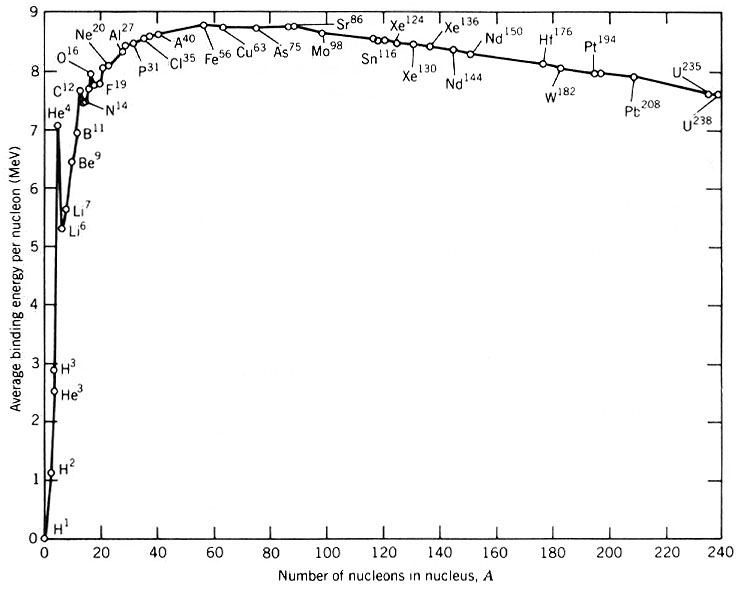
\includegraphics[width=\textwidth]{binding_energy.jpg}
\caption{Binding energy per nucleon. The peak is Fe-56, which is the most stable isotope. \label{f:be}}
\end{center}
\end{figure}

So, what happens when you get a massive iron core? At this stage, the electrons are fully degenerate, but it's good to note that not all the pressure comes from degeneracy, since the core temperature is still quite high (probably close to $10^{10}-10^{11}~{\rm K}$. The core starts to contract, as it did at the end of every other burning phase. As a result, the temperature increases, but this time, there is no other isotope we can fuse iron into and extract energy to re-expand the core. Instead, the temperature continues to increase until photons are energetic enough to start photodissociating iron nuclei into alpha particles and neutrons and photodissociating alpha particles into neutrons and protons. This robs the core of some of its pressure support, which is a combination of thermal and photon pressure, because a bunch of photon energy goes into breaking these nuclei apart. Note that this effect is more important in more massive stars, which have higher core temperatures. Meanwhile, neutronization has been happening at the same time. This starts occurring during Si burning, but when the Fe core grows very massive, it can produce a runaway that saps the core of its electron degeneracy pressure. The neutronization (which is through inverse beta decay), removes electrons and therefore reduced the electron degeneracy pressure. This is what eventually causes the core to collapse rapidly to a neutron star. This also ``deleptonizes" the core by sending out neutrinos, which don't interact much with matter and escape rapidly at this state. The timescale for this collapse is roughly the freefall timescale
\begin{equation}
\tau_{ff} \approx (G\rho)^{-1/2} \approx \biggl(\frac{GM}{R^3}\biggr)^{-1/2} \approx \biggl(\frac{G{\rm M}_\odot}{(6\times 10^8~{\rm cm})^3}\biggr)^{-1/2} \approx 1.2~{\rm s}\,\,.
\end{equation}
Some people quote the freefall time as 0.1-0.5 s, so this gets it to an order of magnitude.

Anyway, now we've rapidly collapsed our entire Chandrasekhar-mass iron core into a neutron star. What happens to everything else? Well, this collapse is much faster than the sound-crossing time of the star. It takes the outer layers a lot more time to ``learn" about the sudden loss of support from below. Note that the core radius is tiny, something like an Earth radius, while the rest of the star may be several to a thousand solar radii. There is not a super sharp cutoff for which layers follow the core and which hang for a bit, but they are basically divided into these two groups. The outer layers of the star then start falling supersonically (I think) toward the core. Meanwhile, the core density roughly equals and surpasses the nuclear density, which is something like $10^{14}~{\rm g}~{\rm cm}^{-3}$. Through rapid collapse, it's overshot its equilibrium as the nuclear strong force takes over pressure support. This causes the core to ``bounce" and the surface moves out a bit very rapidly, right into the falling outer layers. This creates a powerful shock that then propagates outward into the still infalling layers of the star. Much of the shock energy goes into thermally heating the layers of the star and dissociating heavy elements as well as causing explosive nucleosynthesis. This is dominated by the production of $^{56}Ni$ because the layers outside the core are mostly symmetric ions, meaning they have the same numbers of protons and neutrons. Nickel is the most energetically favorable nucleus under the conditions of this rapid nucleosynthesis of symmetric matter, whereas iron was most favorable when there were more neutrons than protons.

The shock has lost a lot of its energy now, even before it reaches the surface. Depending on the energy in the shock, the density of the material, and the radius of the star (i.e. how much matter the shock needs to get through), it will most likely stall. This may not be the case for low-density matter and small radii, but for Type II supernovae (big hydrogen layer) it's very likely. Through some mechanism, we need to revive the shock if we want an explosion.

Meanwhile, the neutron star is super hot and is cooling by releasing neutrinos. These come from the inverse beta decay processes that have been happening before and during collapse:
\begin{equation}
e^- + p \rightarrow \nu_e + n\,\,.
\end{equation}
In fact, this is where most of the energy from the core collapse goes. If we calculate the difference between the gravitational binding energy of the pre-collapse core and the resulting proto-NS, it's about $10^{53}$ ergs! Spoiler alert---that's 100 times as much as the energy we actually see coming out of a supernova based on its line velocities and luminosity. It seems like the best way to reconcile all this is to somehow get 1\% of the energy from neutrinos deposited into the outer layers of the collapsing star in order to revive the shock and get an explosion as we observe. It's not a crazy idea, since the densities become so high that neutrino interactions should be important but we still haven't really pinned this down. There are a couple other possible explanations for how to revive the shock, such as through fluid instabilities, but neutrinos seem like the most viable way right now. Eventually the supernova enters a phase of homologous expansion, which for a fluid element is described by $r = v t$. Everything is expanding at a constant rate, and things that are moving away from the explosion site faster are farther from it proportionally. This holds until the ISM gets in the way (see the ISM section for later phases of supernova remnant expansion).

Okay, we've successfully blown up our star. What do we expect to see? The first thing should be what's called ``shock breakout". This is just when the shock reaches the surface of the star, and there should be a burst of high-energy radiation associated with that. So far it hasn't been observed because it occurs on a very short timescale (I would say minutes to hours), and we'd have to be pointing directly at the supernova while this happens. Then it goes dark---a lot of energy has just been deposited into the outer layers of the star, but it's so dense that the photons haven't had time to diffuse out yet. When they do, there is a gradual rise to roughly peak brightness over the course of a few days to a week.

This is where supernovae from stripped-envelope stars (SNe Ib, Ic) differ from stars that mostly still have their big fat layer of hydrogen (SNe II). For stars without this envelope, energy deposited directly from the shock is not that significant for powering the supernova light curve. Instead it is mostly the decay of $^{56}{\rm Ni}$ to $^{56}{\rm Co}$ (half life $\sim 6$ days to $^{56}{\rm Fe}$ (half life $\sim 80$ days) that supplies all the power. These are beta decays accompanied by gamma-ray emission in the center of the explosion near the proto-NS, and these gamma-rays are thermalized in the ejecta and the energy is re-emitted partly at optical wavelengths, which is why we see this energy come out in the optical. The relationship between the observed peak of the supernova and the is given by Arnett's law, which assumes that the luminosity at peak is given roughly by the total amount of nickel produced (I should find a good expression of Arnett's law and put it here). Anyway, at first the ejecta expands adiabatically and we don't see much because all these photons are trapped inside. Once the photon diffusion time roughly equals the time since explosion, all these photons start to escape, and then the light curve dips to follow the cobalt decay tail (see Figure \ref{f:sn_lc}

For Type II supernovae, the story is a bit different. Here the ejecta are dominated by a thick hydrogen layer (of course, there will be some situations in between these and Ib types, so you could have sort of hybrid cases). The shock-heated ejecta expand adiabatically as before, and radioactive decays are still depositing photons into the ejecta, which we can't see yet. Then the luminosity goes up as the ejecta expands---however, the luminosity is mediated not immediately by radioactivity but by hydrogen recombination.

\begin{figure}[!h]
\begin{center}
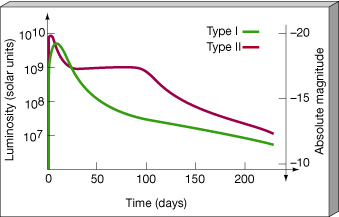
\includegraphics[width=\textwidth]{sn_lc.jpg}
\caption{Approximate light curves for Type I and Type II supernovae. \label{f:sn_lc}}
\end{center}
\end{figure}

Hydrogen recombines at roughly a single temperature (check what this is). As we look at the ejecta, it starts out ionized, but the temperature in the outer layers drops to the recombination temperature, and the opacity drops dramatically. In the optical, at least, we basically see down to where the hydrogen is recombining. This front moves inward in comoving (or mass) coordinates, as more of the inner layers cool---but the layers are also moving outward in real space coordinates. The net effect is that the radius at which most of your light is being emitted stays roughly the same. The temperature also stays roughly the same, so this results in a ``plateau" in luminosity for about 100 days. After we've seen through the entire hydrogen layer, which has become optically thin, the light curve proceeds in a way similar to Type I supernovae, following a cobalt decay tail (again see Figure \ref{f:sn_lc}.

Now let's talk about thermonuclear supernovae, the most common of which are Type Ia supernovae. These come generally from C/O-dominated white dwarfs that are close to the Chandrasekhar mass. Contrary to popular belief, they don't generally blow up quite at the Chandrasekhar mass. This is just the maximum mass a white dwarf can have before relativistic electron degeneracy pressure can no longer support it. What actually matters is when you're allowed to unstably burn carbon. 

The general picture people have on how to get a white dwarf under such conditions encompasses two possibilities: single-degenerate (white dwarf accretes from a normal star that has overflowed its Roche lobe, probably depositing hydrogen) and double-degenerate (two white dwarfs merge or collide). There is some debate about which is more likely or whether you can have one or the other, but it's probably one of these two situations. The important thing is that you get your white dwarf up to a certain mass, meaning you get certain temperatures and densities in the center. Once the temperatures and densities are high enough, carbon burning starts (and to some extent oxygen), and this fuels some confection and a deflagration flame. The physics isn't very well known at this point, and there are a few different theories I won't go into about how this actually ends up disrupting the star. But basically you end up with a runaway reaction in which carbon is burning and raising the temperature, which doesn't actually change the pressure support in the star because the pressure is dominantly from degenerate electrons. This causes a runaway, pretty analogous to the helium flash, and at some point this runaway carbon burning turns from a subsonic deflagration into a supersonic detonation, but we currently aren't that clear on how this happens.

This burning of carbon and oxygen to heavier elements ends up being enough to unbind the star, obliterating it completely (whereas in core-collapse supernovae there is a remnant left behind). Sort of surprisingly, it turns out that the total energy is similar to that released in core-collapse supernovae (not in neutrinos), about $10^{51}~{\rm ergs}$. The luminosity is somewhat more than for core-collapse supernovae, $\sim10^{43}~{\rm ergs}~{\rm s}^{`-1}$ rather than $\sim10^{42}~{\rm ergs}~{\rm s}^{`-1}$, so these are the most commonly observed supernovae even though core collapse are actually more common.

These supernovae are, like other Type I supernovae, powered predominantly by radioactive decay, and so their light curves look very similar to those of SNe Ibc, although generally brighter and over a longer timescale (i.e. more nickel is formed in these explosions).

One thing we don't know is what happens if a white dwarf gets dense enough in its center for electron capture to happen before you can start runaway carbon burning. This is more likely for O/Ne/Mg white dwarfs, since electron capture onto Mg and Ne is easier than onto C and O (and C is what you need to burn unstably). These should come from intermediate ZAMS mass stars, $6-8$ or $8-10$ solar masses, depending on whom you ask. In this case, the white dwarf could theoretically collapse to a neutron star and create a really weak explosion, which is the topic of io's research. :)

\textbf{Good numbers to know} about normal supernovae of any type: $E \sim 10^{51}~{\rm ergs}$, $M_{\rm ej} \sim 1~{\rm M}_\odot$, $L \sim 10^{42-43}~{\rm ergs}~{\rm s}^{`-1}$, $v_{\rm ej} \sim 10,000~{\rm km}~{\rm s}^{-1}$.

\subsection{Neutron Stars}

\subsection{Black Holes}

The first thing to know about black holes is that their escape velocities are greater than the speed of light. The hand-wavey way to derive the Schwarzschild radius is to set the gravitational potential energy $\frac{-G Mm}{r}$ equal to the kinetic energy of a classical particle orbiting it $\frac{1}{2}m v^2$, then setting the orbital velocity equal to the speed of light. This gives the result
\begin{equation}
R_s = \sqrt{\frac{2GM}{c^2}}\,\,.
\end{equation}
Of course, the real way to derive this radius is using general relativity, but I think this approach will suffice. Note: if you try to derive this by setting the gravitational force equal to the centripetal force experienced by the particle, you will be off by a factor of two.

The mean density of a black hole is given approximately by finding $\frac{M}{R_s^3}$, which is roughly
\begin{equation}
\frac{M}{\biggl( \frac{GM}{c^2} \biggr)} \approx 6 \times 10^{17} \biggl(\frac{M}{{\rm M}_\odot} \biggr)^2~{\rm g}~{\rm cm}^{-3}\,\,.
\end{equation}
This density is important for determining how important tidal dissipation is. For the tidal force, imagine a body of mass $M$ tidally pulling on a smaller mass $m$ at a distance $r$. Say the small mass can be divided into two masses $\frac{m}{2}$ separated by a distance $h$, which would be about the radius of the small mass. The force required to pull this mass apart is about $\frac{G (m/2)}{h^2}$. The tidal force is given by
\begin{equation}
\frac{GM(m/2)}{(r + h)^2} - \frac{GM(m/2)}{r^2} \approx \frac{GM(m/2)h}{r^3} > \frac{G(m/2)^2}{h^2}
\end{equation}
is the condition for tidal dissipation (note: there was some expansiony math stuff that happened here that I'm not sure about. I think it works if you just multiply out and take the largest term on the top and bottom). This gives us
\begin{equation}
\frac{M}{r^3} > \frac{m}{h^3}\,\,,
\end{equation}
so the densities of both the disrupting black hole and the small mass determine whether tidal disruption can happen.

Spins of black holes:

Let's look at the angular momentum at maximal spin. This we can approximate by treating the system semi-classically and just using $v = c$ and the Schwarzschild radius
\begin{equation}
J \sim Mc \frac{GM}{c^2} \sim \frac{GM^2}{c} = 9 \times 10^{48} \biggl( \frac{M}{{\rm M}_\odot} \biggr)^2 ~{\rm g}~{\rm cm}^2~{\rm s}^{-1}\,\,.
\end{equation}
By comparison, for a maximally rotating Main-Sequence star,
\begin{equation}
J_* \approx \sqrt{G M_* R_*} M_* \approx 6 \times 10^{51}\biggl( \frac{M_*}{{\rm M}_\odot} \biggr)^2 ~{\rm g}~{\rm cm}^2~{\rm s}^{-1}
\end{equation}
and for a galaxy:
\begin{equation}
J_{\rm gal} \approx \sqrt{G M_{\rm gal} R_{\rm gal}} M_{\rm gal} \approx 10^{74}~{\rm g}~{\rm cm}^2~{\rm s}^{-1}\,\, ,
\end{equation}
assuming the radius is about $10~{\rm kpc}$ and the mass is about $10^{11}~\rm{M}_\odot$.

The Schwarzschild metric:

Here we get to break out some fun GR notation. The gravitational field around a nonrotating black hole is described by the Schwarzschild metric, which is given by (note it is customary to set $G = c = 1$)
\begin{equation}
-d\tau^2 = ds^2 = -\biggl( 1 - \frac{2M}{r} \biggr) dt^2 + \frac{dr^2}{1 - \frac{2M}{r}} + r^2(d\theta^2 + \sin^2\theta) d\phi^2\,\,.
\end{equation}
In real units, this can be rewritten as
\begin{equation}
-c d\tau^2 = -\biggl( 1 - \frac{R_s}{r} \biggr) c^2 dt^2 + \frac{dr^2}{1 - \frac{R_s}{r}} + r^2(d\theta^2 + \sin^2\theta) d\phi^2\,\,.
\end{equation}
Here $r$ is the circumferential length. At a fixed point, $dt = \frac{d\tau}{\sqrt{1 - \frac{2M}{r}}}$. 

Let's look at orbits in this metric. Set $\frac{\partial}{\partial t} = 0$ and $\frac{\partial}{\partial \phi} = 0$ (not sure why). Define $e = -u_0 = $ constant and $h = -u_\phi =$ constant. We have
\begin{equation}
e = -u_0 = -g_{00} u^0 = -g_{00} \frac{dt}{d\tau} = \biggl( 1 - \frac{2M}{r} \biggr) \frac{dt}{d\tau}\,\,,
\end{equation}
\begin{equation}
h = -u_\phi = g_{\phi \phi} u^\phi = r^2 \frac{d\phi}{d\tau}\,\,.
\end{equation}
We've defined these orbits to remain in the plane $\theta = \frac{\pi}{2}$, so $u^\theta = 0$.
\begin{equation}
g_{\alpha \beta}u^\alpha u^\beta = -1 \rightarrow g_{00} (u^0)^2 + g_{rr}(u^r)^2 + g_{\phi \phi} (u^\phi)^2 = -1
\end{equation}
and this can be rewritten as
\begin{equation}
g^{00} (u_0)^2 + g_{rr}(u^r)^2 + g^{\phi \phi} (u_\phi)^2 = \frac{1}{g_{00}} e^2 + \frac{1}{1 - \frac{2M}{r}}(u^r)^2 + \frac{1}{g_{\phi \phi}} h^2 = -1
\end{equation}
The important take-away equation is then:
\begin{equation}
\biggl(\frac{dr}{d\tau} \biggr)^2 = e^2 - \biggl( 1 - \frac{2M}{r} \biggr) \biggl( 1 + \frac{h^2}{r^2} \biggr)\,\,,
\end{equation}
where the second term (not $e^2$) is the effective potential $V_{\rm eff}$. A plot of this potential (the square root of it) is shown in Figure \ref{f:veff}. The equilibrium points are shown with black dots, but the inner ones are unstable. The curve with the equilibrium point that reaches 1 has the same potential energy at infinity, so this represents a particle that comes from infinity, approaches this radius, and then goes back out to infinity.


\begin{figure}[!h]
\begin{center}
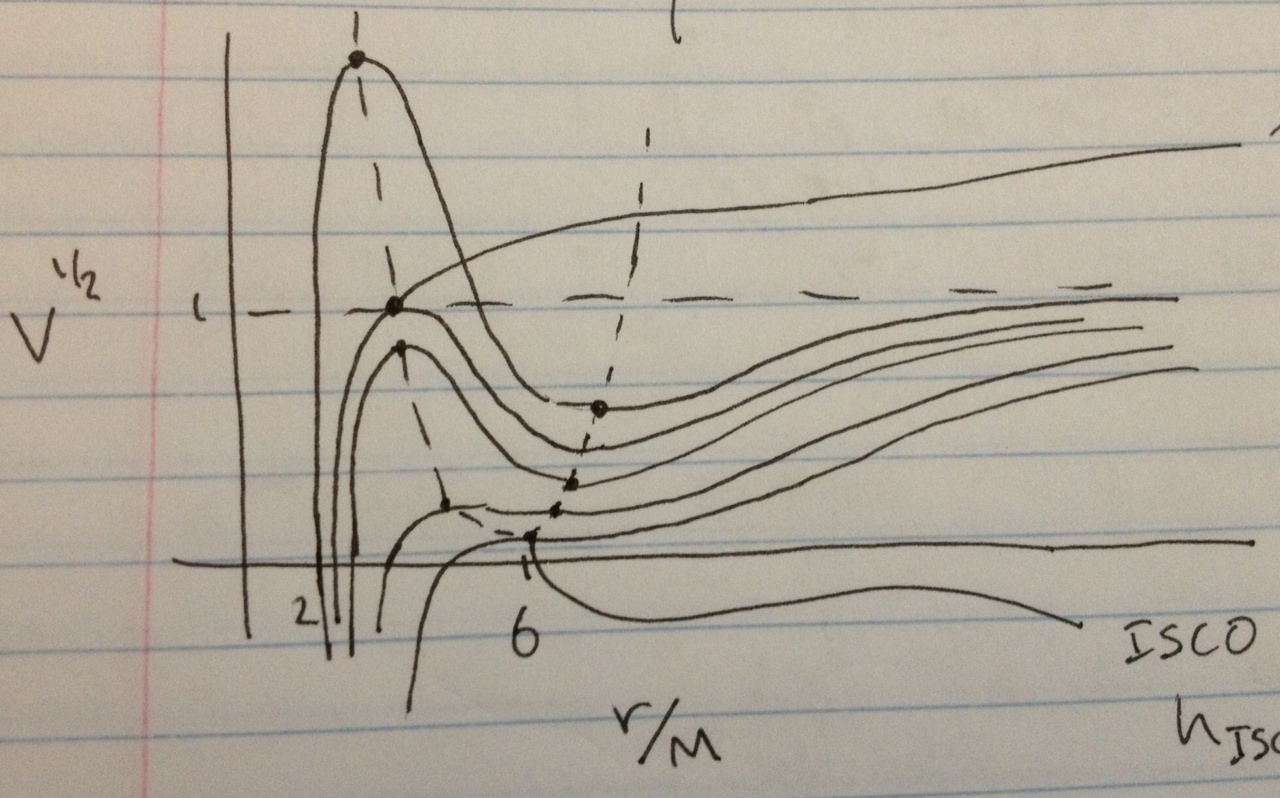
\includegraphics[width=\textwidth]{veff.jpg}
\caption{Effective potential versus radius around a Schwarzschild black hole. The innermost stable circular orbit (ISCO) is marked at $r = 6M$ \label{f:veff}}
\end{center}
\end{figure}

I have in my notes that if you have an accretion disk around your black hole, the energy you get out is the gravitational binding energy of the matter at the innermost stable circular orbit. I'm not sure why in infall from $R_{ISCO}$ doesn't count, though.


This is the potential for massive particles. For massless particles like photons, the orbits are described instead by
\begin{equation}
\biggl(\frac{dr}{d\lambda} \biggr)^2 = e^2 - \biggl( 1 - \frac{2M}{r} \biggr)  \frac{h^2}{r^2}\,\,.
\end{equation}
Here $e^2$ describes the energy and $\frac{h^2}{r^2}$ describes the momentum. Let's divide by $h^2$ to get
\begin{equation}
\frac{1}{h^2} \biggl( \frac{dr}{d\lambda} \biggr)^2 = \frac{e^2}{h^2} - \biggl( 1 - \frac{2M}{r} \biggr) \frac{1}{r^2} = \frac{1}{b^2} - \biggl( 1 - \frac{2M}{r} \biggr) \frac{1}{r^2}\,\, ,
\end{equation}
where $b$ is the impact parameter. The effect of this is that you can bend photons around black holes many times, and they can spiral around the black hole before either escaping or getting absorbed. See Figure \ref{f:veff_phot} for a plot showing the shape of the potential for photons. In this way, you can, for example, see both polar caps of a neutron star (this treatment applies outside a nonrotating NS as well), and this will affect the light curves of X-ray binaries, among other things.

\begin{figure}[!h]
\begin{center}
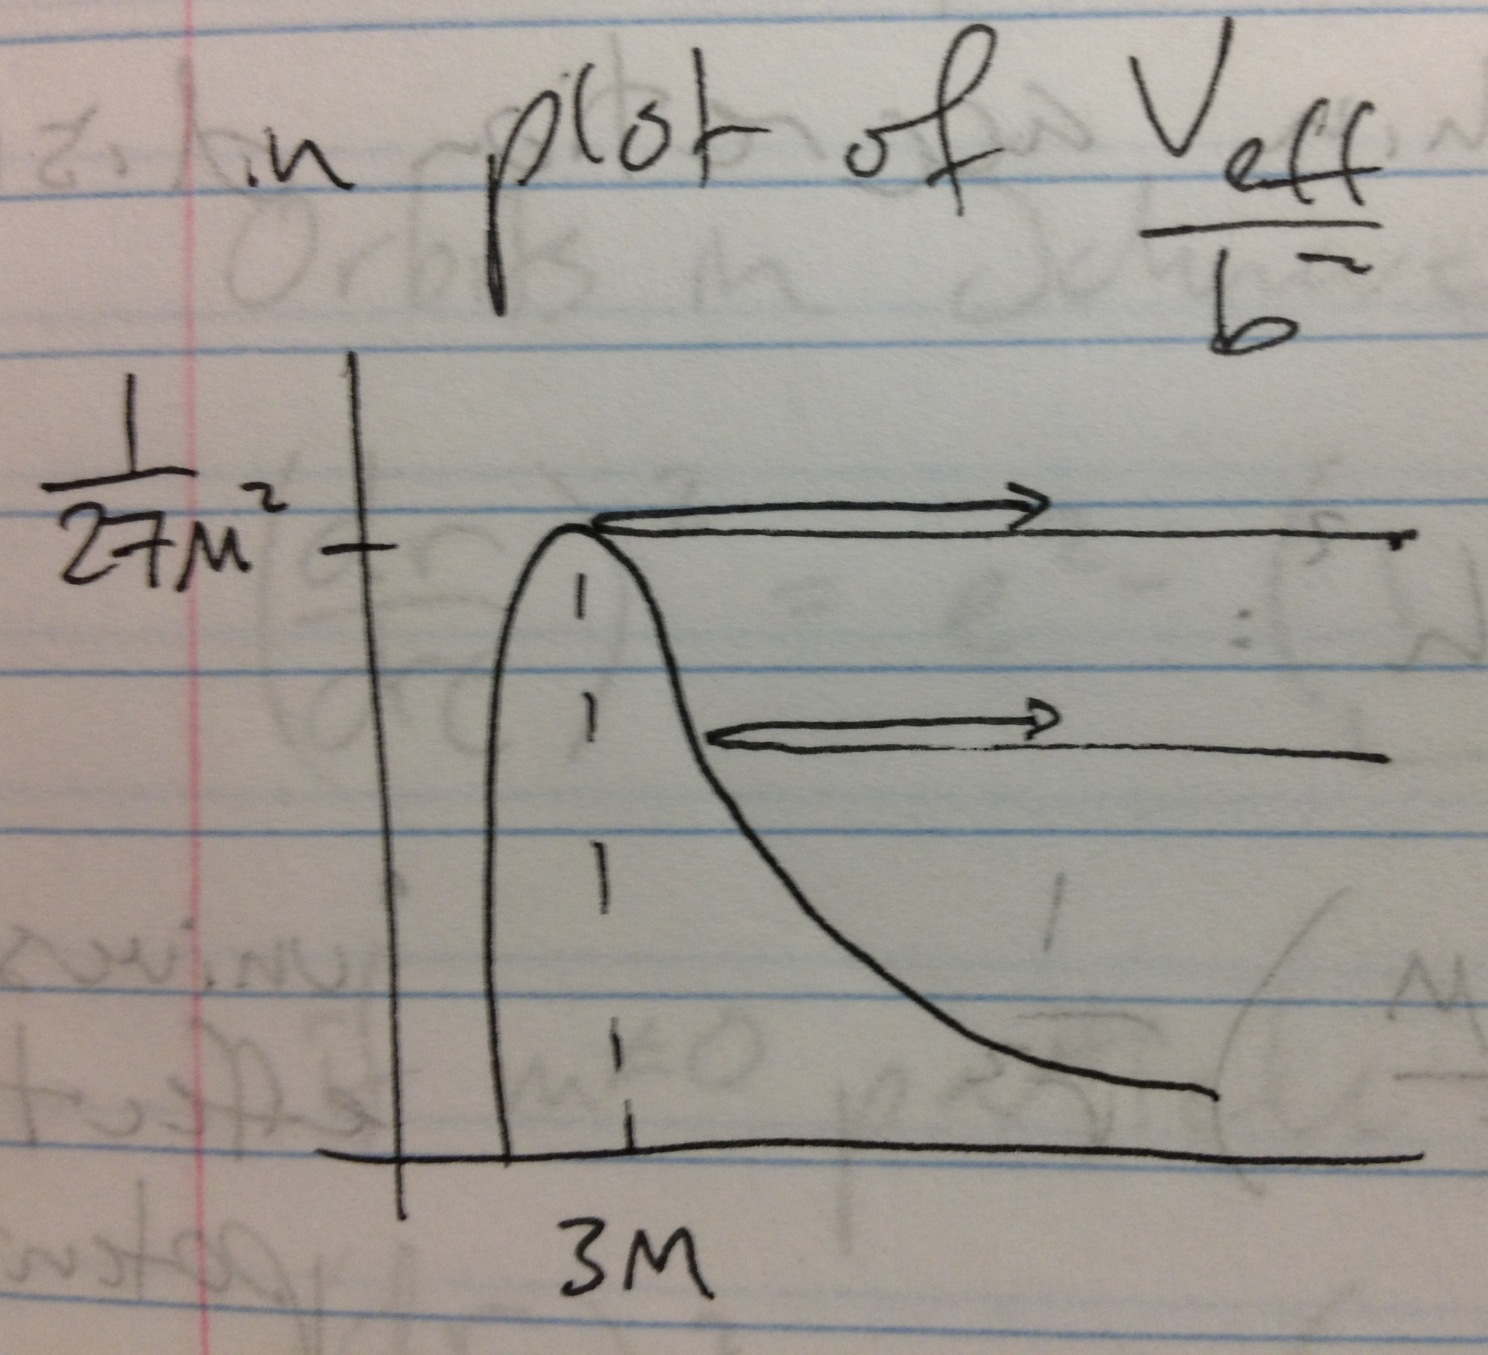
\includegraphics[width=\textwidth]{veff_phot.jpg}
\caption{Effective potential divided by squared impact parameter for a photon around a Schwarzschild black hole. The arrows show tracks of photons coming in from infinity and then escaping. The one that barely makes it to the peak will orbit the black hole many times before escaping. \label{f:veff_phot}}
\end{center}
\end{figure}

\begin{figure}[!h]
\begin{center}
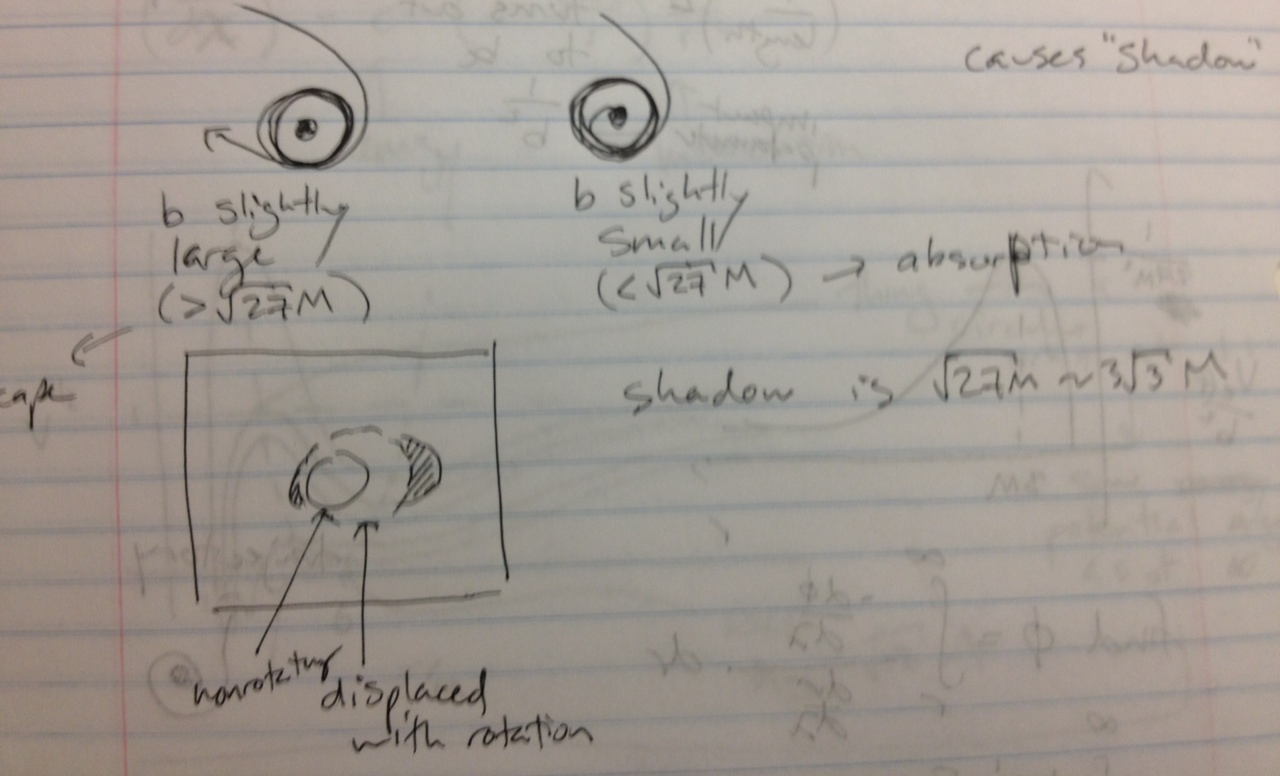
\includegraphics[width=\textwidth]{bh_shadow.jpg}
\caption{Black hole shadow. \label{f:bh_shadow}}
\end{center}
\end{figure}

Rotating Black Holes:

Hopefully we don't need to know too much about this. There's some stuff in my notes about precession as disk warping, but I'll skip it for now and maybe put it in later. The basic thing you should know is that a rotating black hole has what's called an ergosphere. The shape is basically a bulging outward from the event horizon perpendicular to the axis of rotation (so kind of like an oblate spheroid). Spacetime is dragged along with the rotation of the black hole, causing what's called ``frame dragging" (also known as the Lense-Thirring effect). This has some interesting consequences for the spins of objects in the ergosphere, and can actually spin them up or down, even though in the object's rest frame where is no torque. It is also possible to extract rotational energy from the ergosphere by dropping something into the ergosphere such that it passes through and comes back out.

The space around a rotating black hole is described by Kerr geometry. The orbit of an object described by $\Omega$ is constrained by $\Omega_{\rm min} < \Omega = \frac{d\phi}{dt} < \Omega_{\rm max}$, where
\begin{equation}
\Omega^{\rm min}_{\rm max} = \frac{ - g_{0\phi} \mp \sqrt{g_{0\phi}^2 - g_{00}g_{\phi\phi}}}{g_{\phi\phi}}
\end{equation}

\subsection{Bondi Accrection}

Bondi accrection, also called spherical accretion, assumes your central object of mass $M$ is accreting isotropically from an ambient medium at infinity with density $\rho_\infty$, temperature $T_\infty$, $v_\infty = 0$, and sound speed $c_{s\infty}^2$. We're looking for a steady state solution, so $\nabla \cdot (\rho \underline{v}) = 0$ and $\frac{1}{2} v^2 + \phi + h = {\rm constant}$, which is Bernoulli's constant. Here, $\phi = \frac{-G M}{r}$, so we're neglecting self-gravity of the accreting fluid. We also have
\begin{equation}
h = \epsilon + \frac{P}{\rho} = \frac{1}{\Gamma - 1}\frac{P}{\rho} + \frac{P}{\rho} = \frac{c_s^2}{\Gamma - 1}\,\, ,
\end{equation}
where $\Gamma = 5/3$ for monatomic gas. Let's define the Bondi radius, which separates regimes where gravity is and is not dominant:
\begin{equation}
r_B = \frac{G M}{c_{s \infty}^2} \,\,.
\end{equation}
Now let's use Bernoulli's equation to relate the quantities when the gas is at infinity to the quantities at some radius $r$:
\begin{equation}
\frac{1}{2} v_r^2 - \frac{G M}{r} + \frac{1}{\Gamma - 1} c_s^2(r) = \frac{1}{\Gamma - 1} c_{s \infty}^2
\end{equation}
since at infinity, both $v_r$ and $\phi$ go to zero. Dividing out $c_{s \infty}^2$, this equation can be rewritten as 
\begin{equation}
\frac{1}{2}\frac{v_r^2(r)}{c_s^2(r)}\frac{c_s^2(r)}{c_{s \infty}^2(r)} - \frac{r_B}{r} + \frac{1}{\Gamma - 1}\frac{c_s^2(r)}{c_{s \infty}^2(r)} = \frac{1}{\Gamma - 1}
\end{equation}
Let's define here the Mach number $\mathcal{M} = \frac{v_r^2(r)}{c_s^2(r)}$. Also write $\rho_* = \frac{\rho}{\rho_\infty}$, and this equation becomes
\begin{equation}
\frac{\Gamma - 1}{2}\mathcal{M}^2 \rho_*^{\Gamma - 1} + \rho_*^{\Gamma - 1} = 1 + \frac{\Gamma - 1}{r_*}\,\, ,
\end{equation}
where $r_* = r/r_B$. We can use the fact that $4 \pi r^2 \rho v_r = \dot{M}$ is a constant with radius to eventually solve for the Mach number as a function of radius. There are lines of solutions, which matter will follow (some are not physical), shown in Figure \ref{f:mach}. The solutions that cross the sonic point ($\mathcal{M} = 1$) represent physical accretion and wind solutions. The descending curve is for accretion, and the ascending curve is for a wind that goes supersonic.

\begin{figure}[!h]
\begin{center}
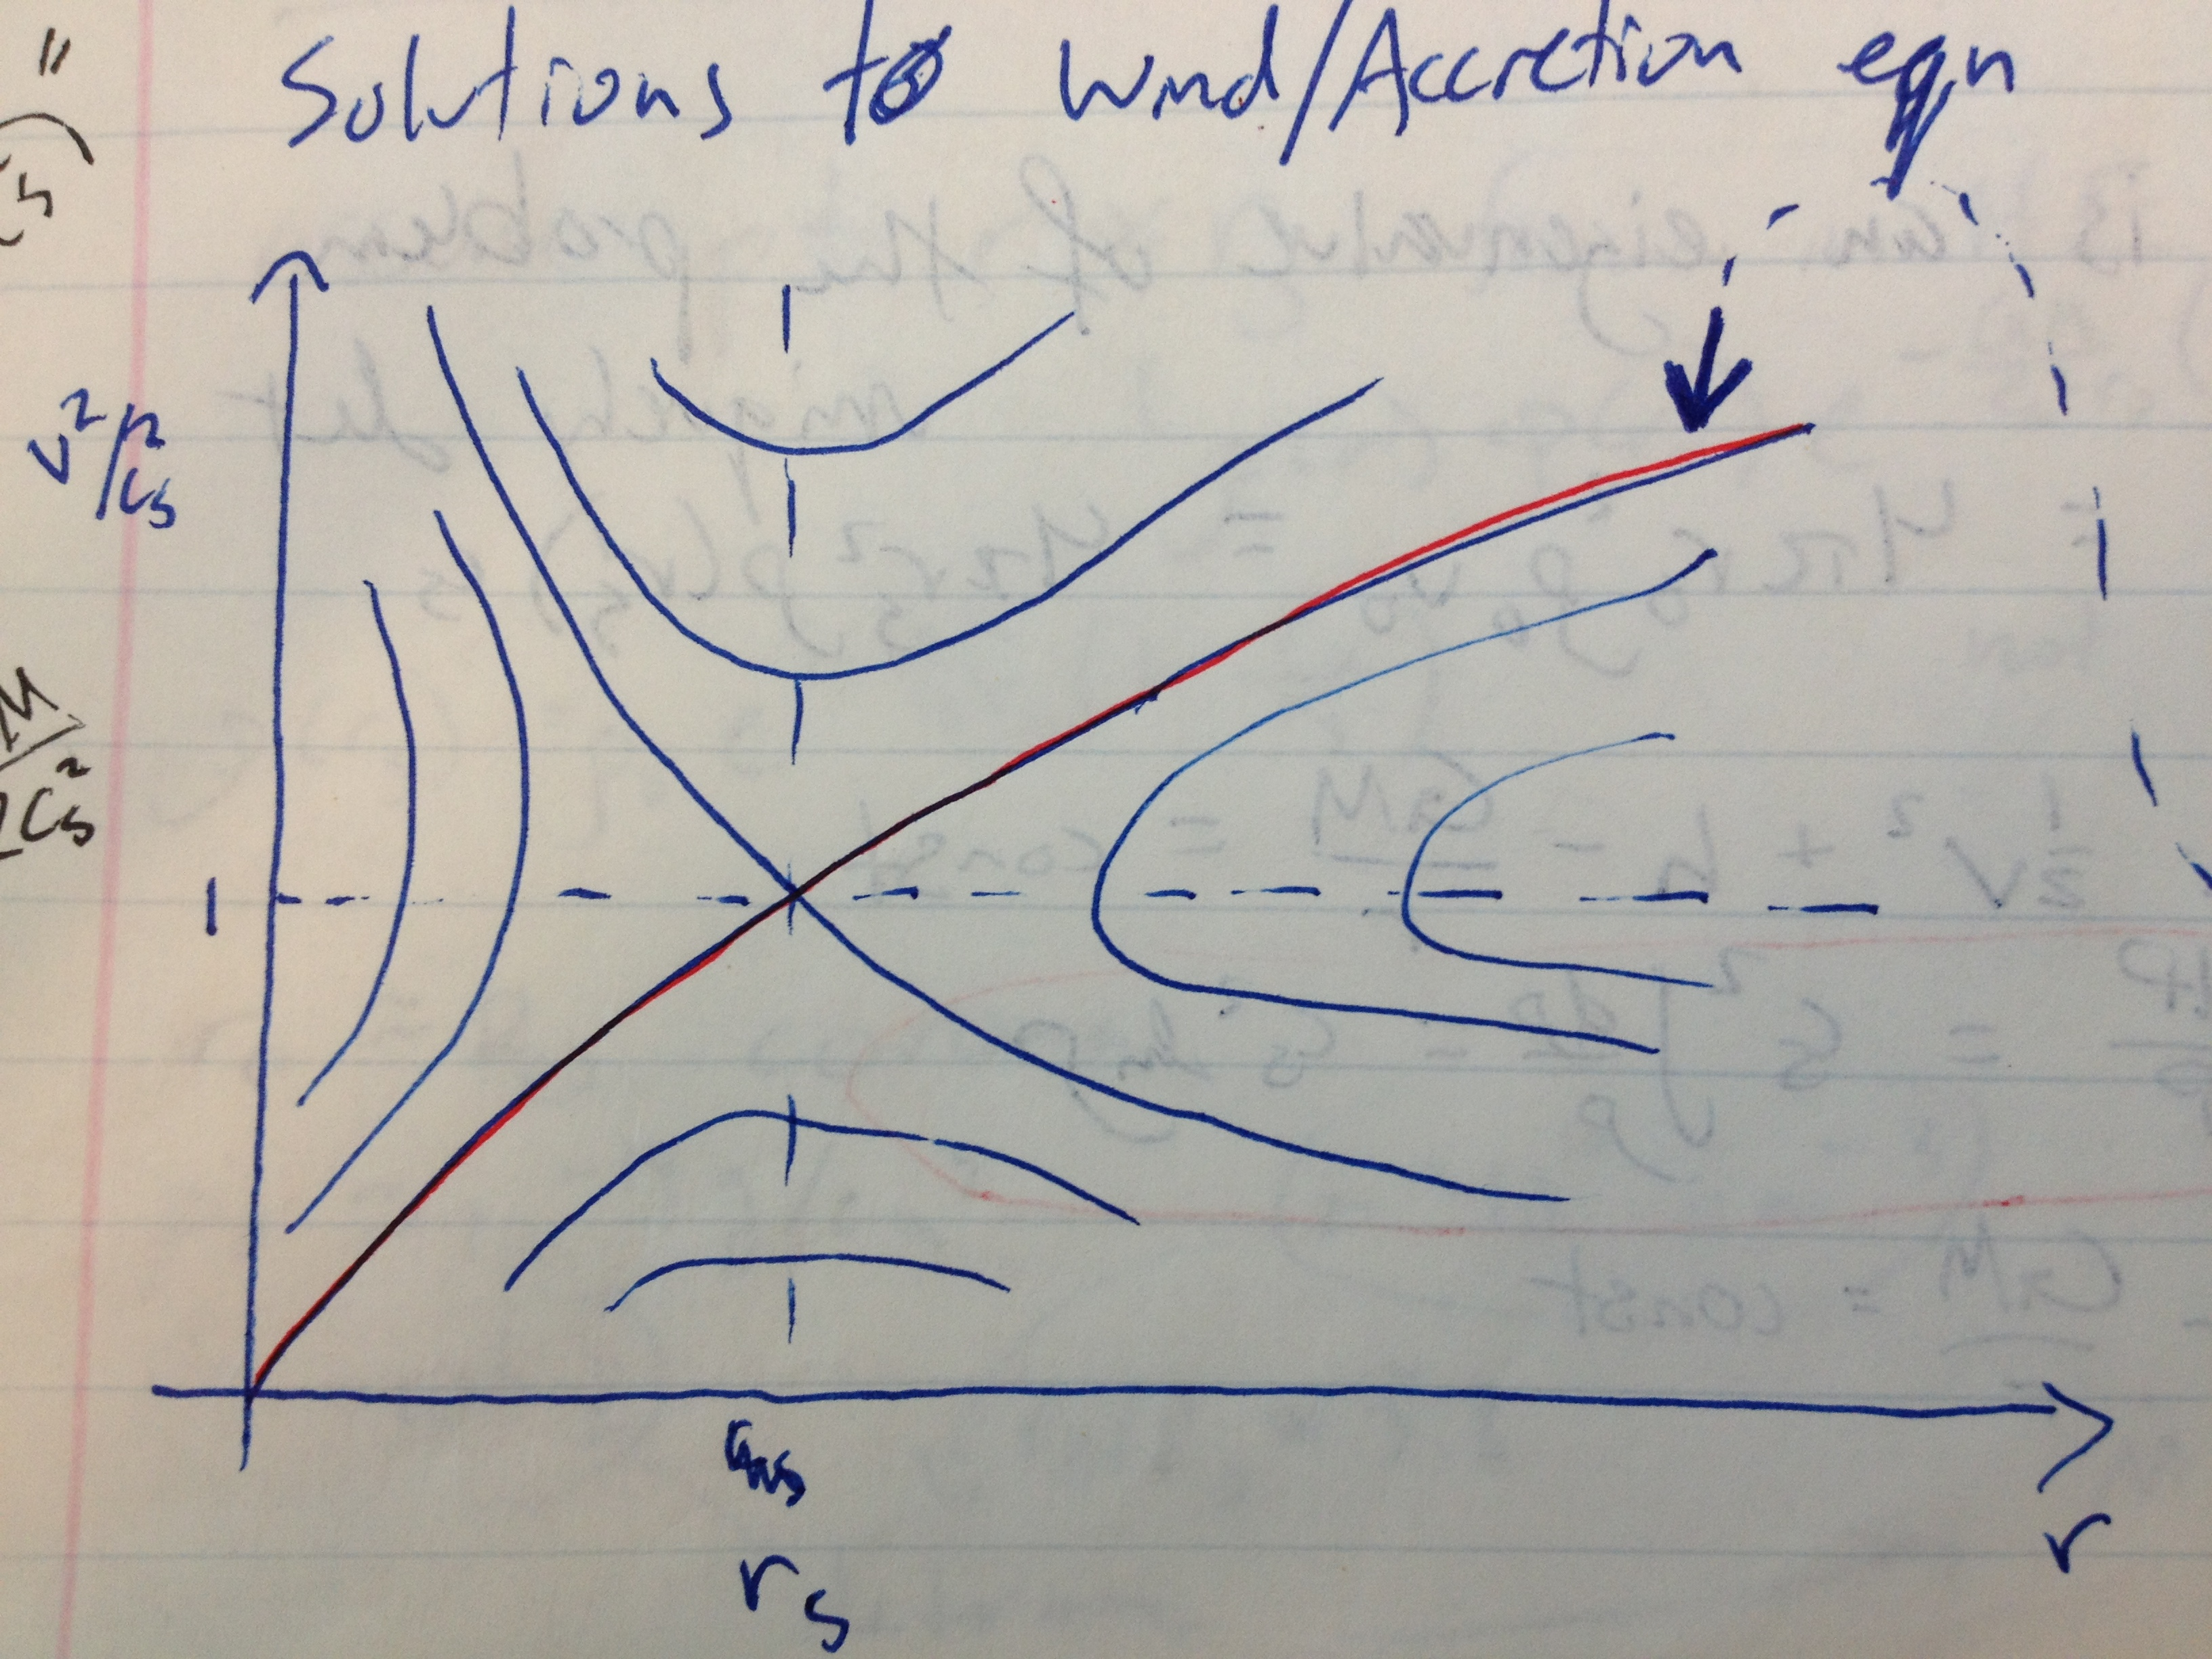
\includegraphics[width=\textwidth]{mach.jpg}
\caption{Mach number as a function of radius showing wind and accretion solutions \label{f:mach}}
\end{center}
\end{figure}

The sonic transition can be used to uniquely define $\dot{M}$:
\begin{equation}
\dot{M} = \lambda 4 \pi \biggl( \frac{G M}{c_{s \infty}^2} \biggr) ^2 \rho_\infty c_{s \infty}\,\, ,
\end{equation}
where $\lambda$ depends on $\Gamma$ and is $0.25$ for $\Gamma = 5/3$, $0.71$ for $\Gamma = 4/3$, $1.12$ for $\Gamma = 1$.

Let's also look at Bondi-Hoyle accretion, which is similar to Bondi accretion, except it's for a mass that's moving through the stuff it's accreting. This time, we can approximate:
\begin{equation}
\dot{M} = \pi \biggl(\frac{2 G M}{v_\infty ^2 + c_{s \infty}^2} \biggr)^2 \rho_* \sqrt{v_\infty ^2 + c_{s \infty}^2}\,\, .
\end{equation}
In this case, the incoming gas (from the perspective of the accreting mass) travels around the object and meets on the other side. This creates a shock in the gas, which heats and expands, and eventually this creates a bow shock around the accreting object as it moves through the fluid.

\subsection{Accretion Disks}

The idea behind accretion disks is that material falls in and maintains the angular momentum it had at large radii, so it starts to orbit the central mass. Viscosity in the disk is what causes it to heat up and radiate, which causes the material to lose energy and start falling in. Let's assume an axisymmetric situation. For Keplertian rotation, $v_\phi = \sqrt{\frac{GM}{r}}$. Because the velocity decreases with radius, we can imagine a thin ring of the disk with an adjacent interior ring moving more slowly and an adjacent outer ring moving more quickly. Imagine elements in these three rings for temporary `bonds' with each other, so the inner ring gets pulled back and bit and the outer ring gets pushed forward a bit due to the interaction between the rings (which is due to viscosity). Actually, the lowest energy state that the disk is trying to get to is one in which a small part of the mass goes out to infinity and carries all the angular momentum with it, while the rest of the accretion disk falls into the accretor.

One good thing to know about an accretion disk is its thickness. The scale height $H$ provides a measure of the thickness when compared with the radius $R$. It's possible to approximate the scale height by using hydrostatic equilibrium in the $z$ direction:
\begin{equation}
\frac{dP}{dz} = -g_z \rho = -\frac{GM}{r^2} \frac{z}{r}\,\,.
\end{equation}
We can hand-wave this by setting $dz = z = H$ and $r = R$ and using ideal gas for $P$:
\begin{equation}
H \sim \biggl( \frac{k_{\rm B} T R^3}{GM m_p}\biggr)^{1/2}\,\,.
\end{equation}
Typical temperatures are around $10^4~{\rm K}$.

Now let's define the surface mass density $\Sigma(r) = \int^\infty_{-\infty} \rho dz$. We can get the average velocity $\langle v_r \rangle$ by integrating $v_r$ over $z$ and $\phi$ in a mass-weighted way. Then we can get the accretion rate,
\begin{equation}
\dot{M} = 2 \pi r \Sigma \langle v_r \rangle\,\, ,
\end{equation}
which is constant with $r$.

Let's look at energy dissipation in the disk. First define the shear $\sigma_{\hat{r}\hat{\phi}} = \frac{1}{2}(v_{x,y} + v_{y,x})$.

(note: I am having trouble condensing this into the important information about accretion disks. If anyone wants to add and restructure, go for it. I'll work on some other things and come back to it later. -io)

\subsection{High-Energy Binaries}

\subsection{GRBs}

\subsection{AGN}

\subsection{Cosmic Rays}
